\chapterpage{Results Analysis and Discussion}
\mychapter{Results Analysis and Discussion}
\label{chap:results}

% This chapter presents and analyses the empirical evidence produced by the implemented components of the proposed adaptive hybrid crowd-counting framework: a pretrained classic person detector, a head detector fine-tuned on the SCUT-Head dataset, a custom four-column multi-column density regression network (Four Column MDNN), a CSRNet style dilated convolution density network, and a classical detection assisted density estimation procedure.

\section{Data Collection and Analysis}

Three annotated datasets underpin the techniques investigated in this research, playing two distinct roles. SCUT-HEAD and ShanghaiTech, Part~B are used to train, fine-tune, and validate the individual learned techniques (the fine-tuned sparse detector and the two dense density-map estimators, respectively). The Public Transport Crowd Counting Dataset (PTCCD) plays a different role: it is not used to train or fine-tune any individual technique, but is instead used to evaluate the performance of the proposed, fully assembled passenger-counting framework under realistic transportation conditions. The two non-learned techniques (the cascade classifier detector and the classical density estimator) rely on pre-existing, general purpose classifiers or on no learned parameters at all, and therefore do not draw on any task specific training or evaluation dataset. Table~\ref{tab:datasets} summarises the three datasets used and the role each plays, and Table~\ref{tab:dataset-stats} reports their detailed size, split, and annotation density statistics as documented by their original sources.

\begin{longtable}{|
    >{\raggedright\arraybackslash}p{0.24\textwidth}|
    >{\raggedright\arraybackslash}p{0.21\textwidth}|
    >{\raggedright\arraybackslash}p{0.15\textwidth}|
    >{\raggedright\arraybackslash}p{0.24\textwidth}|
}
\caption{Datasets used to train and/or evaluate the techniques investigated in this study.}
\label{tab:datasets}\\
\hline
\textbf{Dataset} &
\textbf{Annotation type} &
\textbf{Used by} &
\textbf{Role} \\
\hline
\endfirsthead

\hline
\textbf{Dataset} &
\textbf{Annotation type} &
\textbf{Used by} &
\textbf{Role} \\
\hline
\endhead

\hline
\endfoot

\hline
\endlastfoot

SCUT-HEAD~\cite{peng2018scuthead} &
Head bounding boxes (YOLO text format) &
Fine-tuned sparse detector &
Fine tuning and validation (detection metrics) \\
\hline

ShanghaiTech, Part B~\cite{Zhu2020} &
Head point locations (\texttt{.mat} files) &
Both learned dense branch estimators &
Training and validation (density-map / count metrics) \\
\hline

Public Transport Crowd Counting Dataset (PTCCD) &
Passenger/head bounding boxes (YOLO text format) &
Proposed passenger-counting framework (full pipeline) &
Held-out evaluation only; not used for training or fine-tuning any individual technique \\
\hline

\end{longtable}

\begin{longtable}{|
		>{\raggedright\arraybackslash}p{0.18\textwidth}|
		>{\raggedright\arraybackslash}p{0.09\textwidth}|
		>{\raggedright\arraybackslash}p{0.18\textwidth}|
		>{\raggedright\arraybackslash}p{0.15\textwidth}|
		>{\raggedright\arraybackslash}p{0.24\textwidth}|}
	
	\caption{Detailed dataset statistics}
	\label{tab:dataset-stats}\\
	
	\hline
	\textbf{Dataset} &
	\textbf{Images} &
	\textbf{Train / Test / Val} &
	\textbf{Annotated instances} &
	\textbf{Notes} \\
	\hline
	\endfirsthead
	
	\multicolumn{5}{c}%
	{{\tablename\ \thetable{} -- continued from previous page}} \\
	\hline
	\textbf{Dataset} &
	\textbf{Images} &
	\textbf{Train / Test / Val} &
	\textbf{Annotated instances} &
	\textbf{Notes} \\
	\hline
	\endhead
	
	\hline
	\multicolumn{5}{r}{{Continued on next page}} \\
	\endfoot
	
	\hline
	\endlastfoot
	
	SCUT-HEAD, Part~A~\cite{peng2018scuthead}
	&
	2{,}000
	&
	1{,}100 / 500 / 400
	&
	67{,}318 heads
	&
	Classroom surveillance imagery; low inter-image variance by design
	\\
	\hline
	
	SCUT-HEAD, Part~B~\cite{peng2018scuthead}
	&
	2{,}329
	&
	1{,}630 / 233 / 466
	&
	41{,}749 heads
	&
	Internet-crawled imagery; higher visual variability
	\\
	\hline
	
	SCUT-HEAD, combined
	&
	4{,}329
	&
	2{,}730 / 733 / 866
	&
	109{,}067 heads
	&
	Union of Part~A and Part~B, as used for fine-tuning in this study
	\\
	\hline
	
	ShanghaiTech, Part~B~\cite{Zhu2020}
	&
	716
	&
	400 / 316
	&
	88{,}272 heads (point-annotated)
	&
	Fixed resolution $768{\times}1024$; approximately 9--578 people per image, mean $\approx 123.6$
	\\
	\hline

	Public Transport Crowd Counting Dataset (PTCCD)
	&
	285
	&
	--
	&
	Approx. 8{,}311 passengers/heads (bounding-box annotated)\footnotemark
	&
	Variable resolution; 2--60 annotated objects per image, mean $\approx 29.16$, median 29; used for framework-level evaluation only, not split into train/test
	\\
	\hline
	
\end{longtable}

\subsubsection{SCUT HEAD Dataset}
The fine tuned sparse detector is trained on SCUT-HEAD, a head detection dataset comprising 4{,}329 images with 109{,}067 annotated head bounding boxes~\cite{peng2018scuthead}. The dataset is collected in two parts that differ in imaging condition and scene variability:

\begin{itemize}
	\item \textbf{Part A:} 2{,}000 images sampled from classroom surveillance video within a single university, with 67{,}318 heads annotated; because classroom scenes recur with limited pose variation, the constituent images were deliberately selected to maximise representative variance. As distributed, Part~A is pre-split into 1{,}100 training, 400 validation, and 500 testing images.
	\item \textbf{Part B:} 2{,}329 images crawled from the internet, with 41{,}749 heads annotated, offering greater visual diversity than Part~A. As distributed, Part~B is pre-split into 1{,}630 training, 466 validation, and 233 testing images.
\end{itemize}

Every annotated head is bounded by an axis aligned box $(x_{\min}, y_{\min}, x_{\max}, y_{\max})$ covering the full head extent, including occluded portions, without extraneous background, following the Pascal VOC annotation convention. In the implementation examined for this study, Part~A and Part~B are pooled into a single combined dataset of 4{,}329 images (2{,}730 for training, 733 for testing) while each image's original split membership is preserved, and a single object class (head) is declared, since the study task is class agnostic head localisation rather than the finer classroom versus internet distinction that motivated the dataset's original two part structure.

\subsubsection{ShanghaiTech Dataset, Part B}
Both learned density estimation techniques are trained and evaluated on Part~B of the ShanghaiTech crowd counting dataset, introduced alongside the multi column convolutional architecture on which one of the two density estimators is based~\cite{Zhu2020}. ShanghaiTech as a whole comprises 1{,}198 images with 329{,}547 annotated head points, split into a dense, internet sourced Part~A (482 images) and a sparser, street-level Part~B (716 images); this study uses Part~B only. Part~B images are all captured at a fixed resolution of $768{\times}1024$ pixels on busy Shanghai streets, officially divided into 400 training and 316 testing images, with per-image counts ranging from approximately 9 to 578 people and a mean of approximately 123.6 people per image, substantially sparser than Part~A (mean $\approx$501 people per image), which was not used in this study. Annotations are provided as a single $(x,y)$ pixel coordinate per head, stored per image in a MATLAB \texttt{.mat} file, rather than as bounding boxes. Both density estimation techniques uses only the official 400-image training subset: a fixed, seeded 90/10 split is drawn from it, giving 360 images for training and holding out the remaining 40 for validation during training; this same 40-image held-out set is subsequently reused as the evaluation set for reported test metrics, so the official 316-image test subset is not used by this technique. During training, this technique additionally applies random-crop augmentation, so the network is fed fixed-size image and density-map crops rather than full frames, whereas the held-out validation/test images are processed at their full $768{\times}1024$ resolution; in both cases the target density map is downsampled by a factor of 8 relative to the input. The other technique uses the official test subset directly as its validation set during training, without a further internal split. Point annotations are not used directly as supervision; both techniques convert them into smoothed density maps prior to training, as described in Section~\ref{sec:dense}.


\subsubsection{Public Transport Crowd Counting Dataset}
\label{sec:ptccd}

Unlike SCUT-HEAD and ShanghaiTech, Part~B, the Public Transport Crowd Counting Dataset (PTCCD) is not used to train or fine-tune any individual technique in this study. Instead, it is used to evaluate the performance of the proposed passenger-counting framework as a whole, in realistic transportation environments. The dataset contains a total of 285 images and 285 corresponding annotation files, resulting in a one-to-one correspondence between images and labels. The images represent different passenger configurations and crowd densities, making the dataset suitable for evaluating both sparse and relatively dense passenger-counting conditions.

The number of annotated objects in each image was calculated from the corresponding label file. For every annotation file, the number of non-empty annotation lines was counted. The resulting statistics are shown in Table~\ref{tab:object_statistics}.
\begin{table}[htbp]
\centering
\caption{Statistics of Annotated Objects per Image}
\label{tab:object_statistics}
\begin{tabular}{lc}
\hline
\textbf{Statistic} & \textbf{Number of Objects} \\
\hline
Minimum & 2 \\
Maximum & 60 \\
Mean & 29.16 \\
Median & 29.00 \\
\hline
\end{tabular}
\end{table}

The dataset contains an average of 29.16 annotated objects per image,
with a median of 29 objects and a range of 2 to 60 objects. This
variation represents different passenger-density conditions and helps
evaluate the model's robustness across varying crowd sizes.

\begin{figure}[htbp]
    \centering
    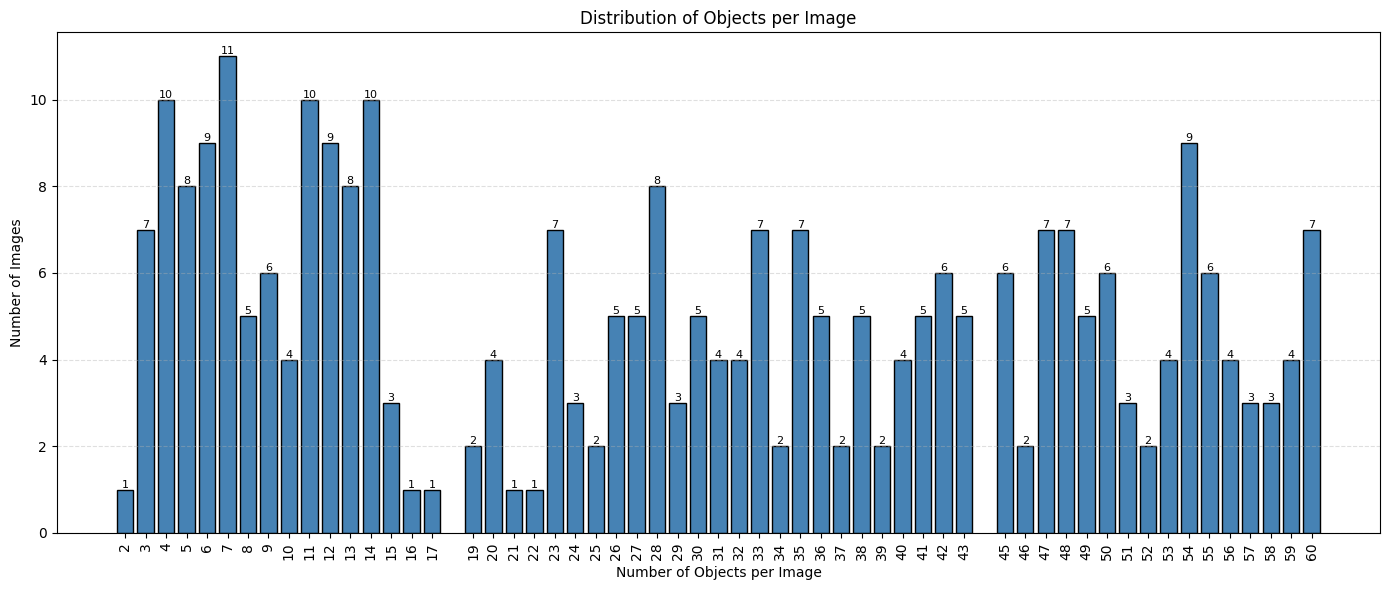
\includegraphics[width=0.90\textwidth]
    {figures/ptccd_image_distribution.png}
    \caption{Distribution of annotated objects per image in the Public
    Transport Crowd Counting Dataset.}
    \label{fig:object_distribution}
\end{figure}

The object-count distribution illustrates the variation in the number
of annotated passengers across the dataset. It provides an overview of
the typical crowd size and the spread of passenger counts among the
images.

\begin{figure}[htbp]
    \centering
    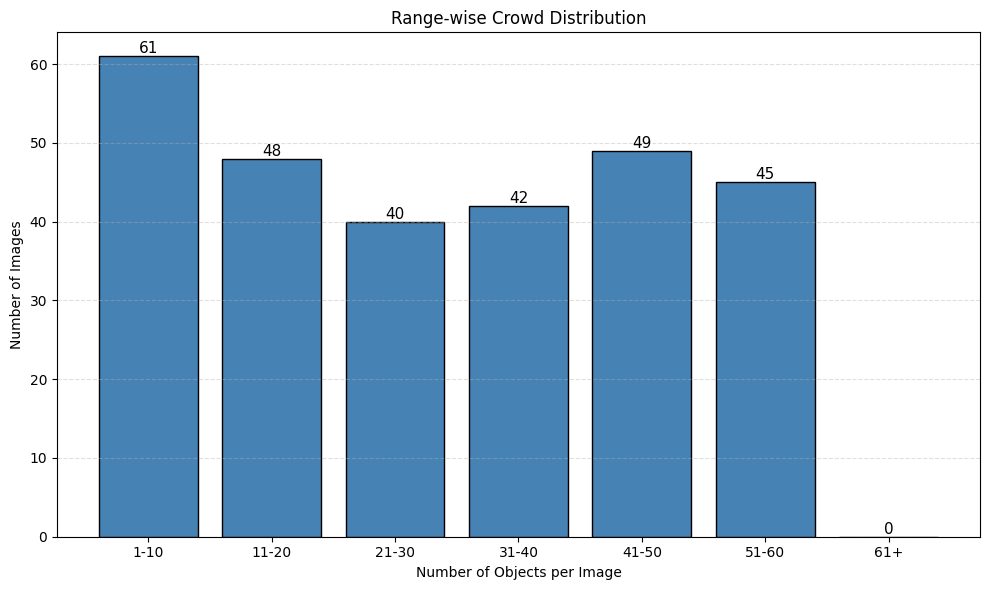
\includegraphics[width=0.90\textwidth]
    {figures/ptccd_range_distribution.png}
    \caption{Range-wise distribution of images based on the number of
    annotated objects.}
    \label{fig:range_crowd_distribution}
\end{figure}

The range-wise grouping provides a simple way to examine whether the
dataset is concentrated around a particular crowd-density level or
contains a broad range of passenger counts. The resulting distribution
is shown in Figure~\ref{fig:range_crowd_distribution}.

\section{Interpretation of Results}

\subsection{Classic YOLO: Pretrained Detector, Qualitative Demonstration}
\label{sec:classic_yolo}

This section reports the experimental results obtained from applying a pretrained, off-the-shelf YOLO object detector to head counting on the same 285-image test set used in the preceding experiments. Detections were obtained using the model's default (pretrained) weights with inference parameters \textit{imgsz=1024}, \textit{conf=0.25}, restricted to \textit{classes=[0]} (the COCO ``person'' category). As the pretrained model was optimised to localise whole body person instances rather than heads, a systematic geometric mismatch between predicted and ground truth bounding boxes is expected \textit{a priori}, independent of the detector's underlying ability to identify the presence of individuals. The results reported below are interpreted with this expectation as the analytical baseline.

\subsubsection{Quantitative Detection Based Counting Performance}

Table~\ref{tab:pretrained_yolo_summary} presents the overall detection performance of the pretrained YOLO detector on the 285-image test set. The very low precision, recall, and F1-score at IoU = 0.50 do not necessarily mean that the detector fails to identify people. The main issue is the difference between the annotations and the detector output: the ground truth contains small head-only boxes, while the pretrained model produces boxes covering the full person. As a result, a correct person detection may have very little overlap with the corresponding head annotation and therefore be counted as a false positive. The low number of true positives is therefore mainly due to this mismatch between the evaluation annotations and the detector's output format.

\begin{longtable}{lc}
\caption{Pretrained YOLO person-detector performance.}
\label{tab:pretrained_yolo_summary} \\
\hline
Metric & Value \\
\hline
\endfirsthead

\multicolumn{2}{c}%
{{\tablename\ \thetable{} -- continued from previous page}} \\
\hline
Metric & Value \\
\hline
\endhead

\hline
\multicolumn{2}{r}{{Continued on next page}} \\
\endfoot

\hline
\endlastfoot

Images & 285 \\
Total Ground Truth & 8{,}310 \\
Total Predictions & 7{,}140 \\
True Positives (IoU 0.50) & 125 \\
False Positives (IoU 0.50) & 7{,}015 \\
False Negatives (IoU 0.50) & 8{,}185 \\
Precision @ IoU 0.50 & 0.0175 \\
Recall @ IoU 0.50 & 0.0150 \\
F1-score @ IoU 0.50 & 0.0162 \\
Mean Ground Truth Count & 29.1579 \\
Mean Predicted Count & 25.0526 \\
Mean Absolute Error (MAE) & 7.2351 \\
Root Mean Squared Error (RMSE) & 9.9359 \\
Mean Absolute Percentage Error (MAPE) & 27.8446\% \\
Pearson Correlation (GT vs.\ Predicted Count) & 0.8704 \\
Coefficient of Determination ($R^2$) & 0.6987 \\

\end{longtable}

The count-level results in Table~\ref{tab:pretrained_yolo_summary} and Figure~\ref{fig:pretrained_yolo_actual_predicted} show that the pretrained YOLO detector performs poorly when its bounding boxes are compared with the head annotations using IoU = 0.50. However, the predicted person counts still show a strong relationship with the actual crowd counts. This suggests that, although the detector does not match the head annotations well at the bounding-box level, it can still provide useful information about the number of people in an image.

\begin{figure}[htbp]
\centering
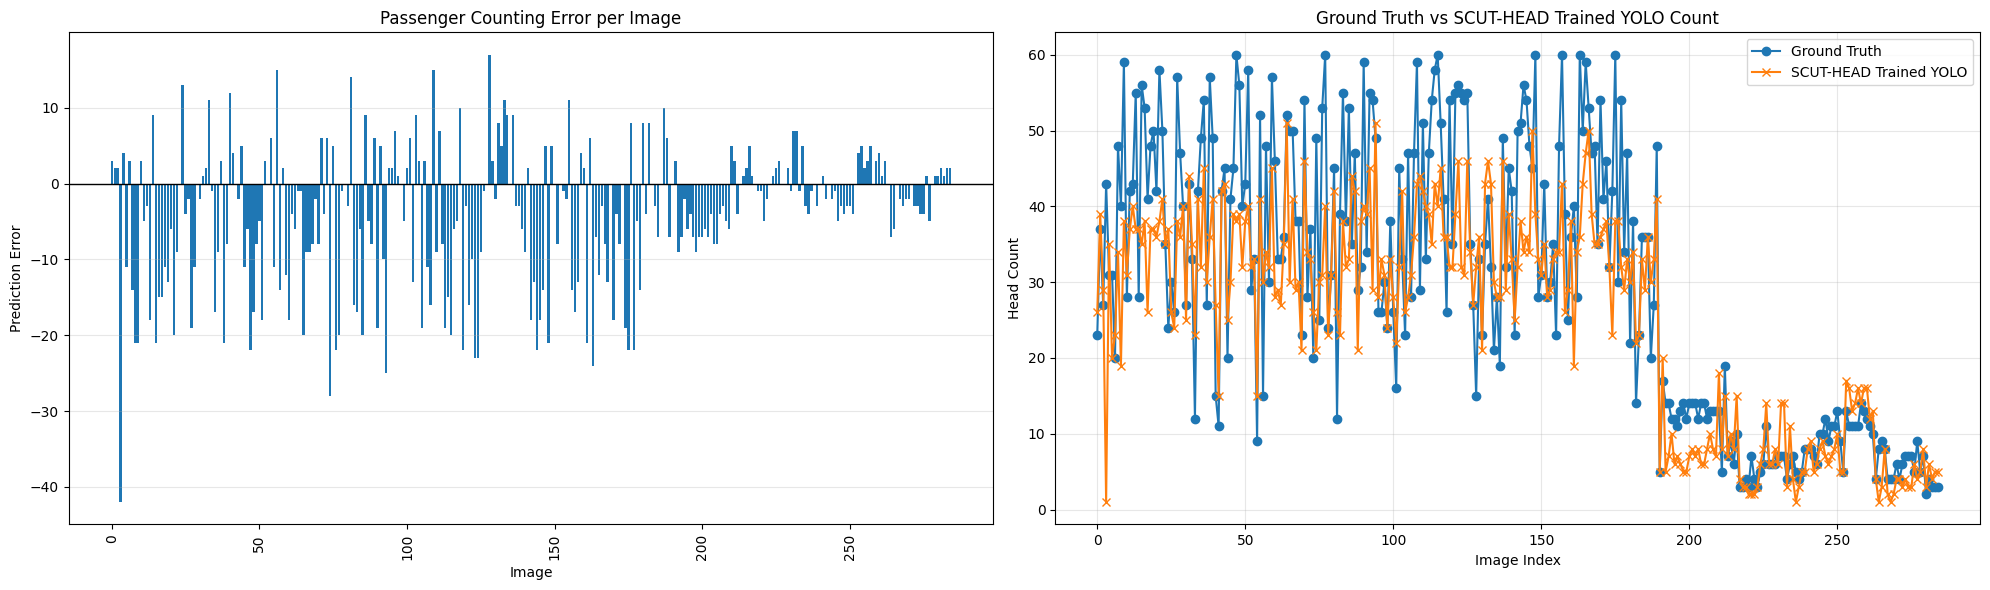
\includegraphics[width=1.0\linewidth]{figures/yolo_pretrained_per_image_error_and_gt_vs_predicted.png}
\caption{Per-image counting error (left) and ground-truth vs. predicted counts (right) for the pretrained YOLO detector.}
\label{fig:pretrained_yolo_actual_predicted}
\end{figure}

The counting error shown in Figure~\ref{fig:pretrained_yolo_actual_predicted} is mainly biased toward underestimation. This is likely due to occlusion in crowded scenes, where people overlap with each other and their full-body bounding boxes can overlap heavily. As a result, non-maximum suppression may remove some detections even when multiple people are present. In contrast, heads can remain visible even when much of the body is hidden. Therefore, the undercounting is mainly related to the use of whole-body detection in crowded scenes rather than a problem specific to this model.

These results show that fine-tuning should focus on adapting the detector to the head-based annotations rather than simply improving its ability to detect people. As discussed in Section~\ref{sec:scut_yolo}, the main issue is the mismatch between whole-person predictions and head-based ground truth. The largest counting error occurred in a highly crowded image where only one person was detected, showing that heavy occlusion can cause severe undercounting as people overlap. This further highlights the need for a head-based detector in crowded scenes.

\subsubsection{Detection-Based Counting Performance by Ground-Truth Count Range}

The results across the six ground-truth count ranges in Table~\ref{tab:pretrained_yolo_range_breakdown} and Figure~\ref{fig:pretrained_yolo_range_metrics} show that absolute counting error generally increases as the crowd becomes larger. However, percentage error is highest in images with fewer people because even a small counting mistake has a larger effect when the ground-truth count is low. Counting accuracy is highest in the moderately populated ranges, where the crowd is large enough to reduce the effect of individual errors but not so dense that occlusion causes major detection problems.

\setlength{\LTcapwidth}{\textwidth}
\begin{longtable}{lccccccc}
\caption{Pretrained YOLO person-detector counting performance by ground-truth count range.}
\label{tab:pretrained_yolo_range_breakdown} \\
\hline
GT Range & $n$ & MAE & RMSE & Mean \% Error & Mean Acc. (\%) & Mean Bias & Mean F1 \\
\hline
\endfirsthead

\multicolumn{8}{c}%
{{\tablename\ \thetable{} -- continued from previous page}} \\
\hline
GT Range & $n$ & MAE & RMSE & Mean \% Error & Mean Acc. (\%) & Mean Bias & Mean F1 \\
\hline
\endhead

\hline
\multicolumn{8}{r}{{Continued on next page}} \\
\endfoot

\hline
\endlastfoot

1--10  & 61 & \textbf{2.1475} & \textbf{2.9113} & 34.9811 & 65.0189 & $-0.3115$ & 0.0903 \\
11--20 & 48 & 5.9583 & 6.9132 & 43.5578 & 57.0672 & 0.6250 & \textbf{0.1312} \\
21--30 & 40 & 4.3250 & 5.7031 & 16.6860 & 83.3140 & 3.2250 & 0.0000 \\
31--40 & 42 & 5.4524 & 7.5325 & \textbf{15.1393} & \textbf{84.8607} & $-2.2143$ & 0.0060 \\
41--50 & 49 & 10.1429 & 12.5966 & 21.9924 & 78.0076 & $-9.6122$ & 0.0008 \\
51--60 & 45 & 16.5778 & 17.5537 & 29.5595 & 70.4405 & $-16.5778$ & 0.0024 \\

\end{longtable}

The counting bias changes with crowd density. In low-density images, the bias is close to zero or slightly positive, indicating that the whole-body detector performs reasonably well when people are mostly visible. In higher-density images, the bias becomes increasingly negative, showing greater undercounting as occlusion increases. This suggests that crowd density has a direct effect on the detector's ability to count people accurately.

\begin{figure}[htbp]
\centering
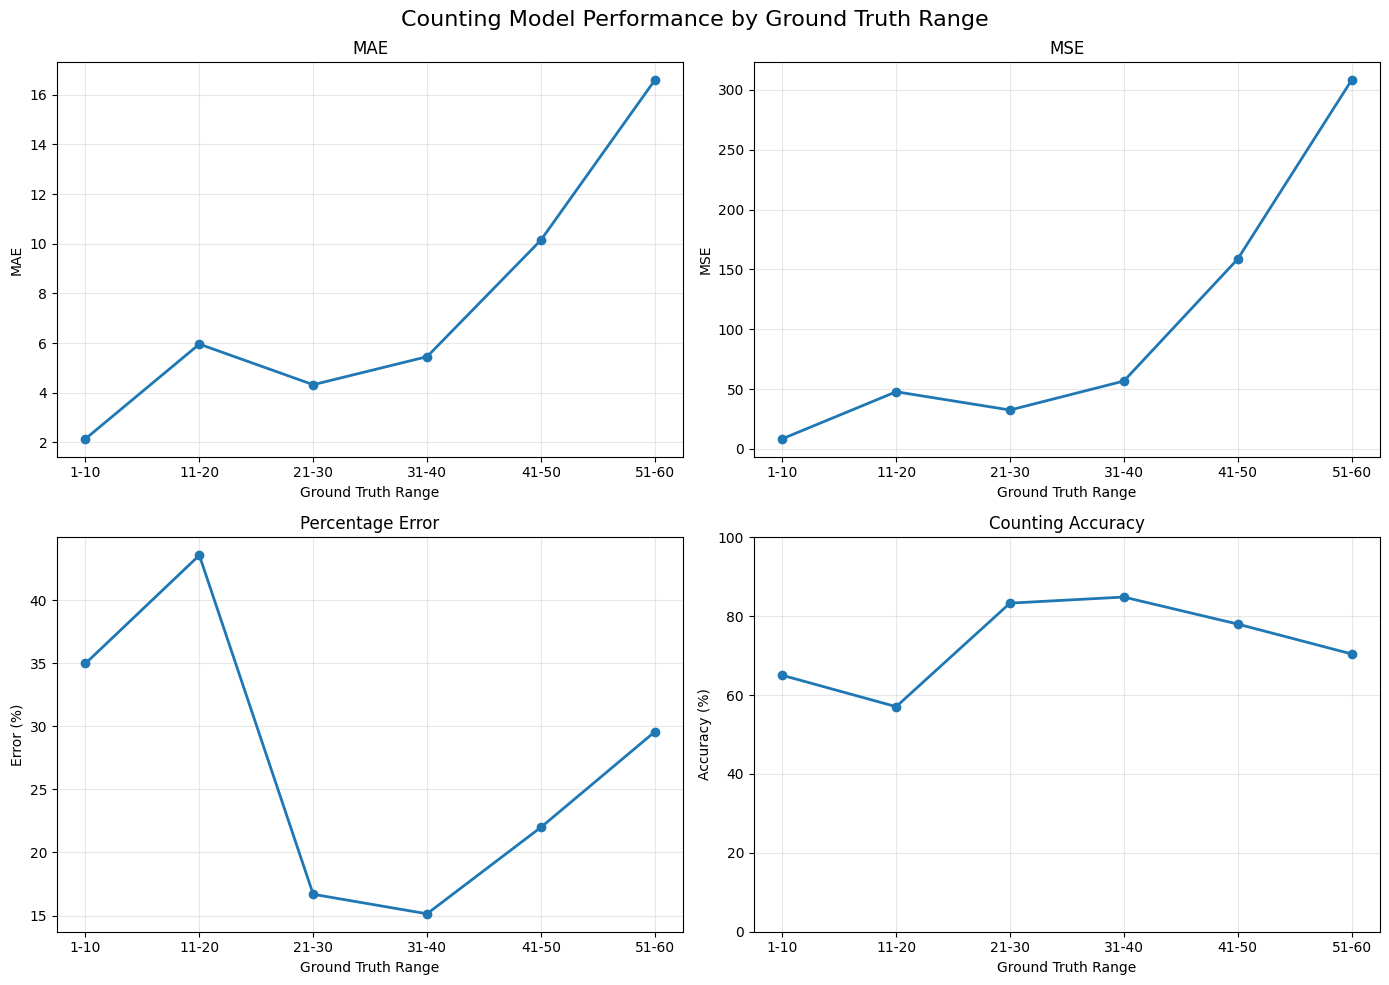
\includegraphics[width=1.0\linewidth]{figures/yolo_pretrained_performance_by_gt_range.png}
\caption{Pretrained YOLO performance across ground-truth count ranges.}
\label{fig:pretrained_yolo_range_metrics}
\end{figure}

Box-level detection performance decreases as crowd density increases and becomes very low in high-density scenes. This is mainly caused by the mismatch between whole-person predictions and head-level annotations, which becomes more severe when people are heavily occluded. As crowd density increases, it becomes harder for whole-body boxes to achieve an IoU of 0.50 with the smaller head annotations.

These results show that the pretrained detector's counting performance depends on crowd density. It performs better in low- to moderate-density scenes but degrades in high-density scenes. This density-related pattern is not clear from the overall box-level metrics, which remain very low across the test set.

\subsection{SCUT-Head YOLO: Fine-Tuned Head Detector}
\label{sec:scut_yolo}

This section reports the experimental results obtained from training and evaluating a YOLO-based object detector on the SCUT-Head dataset for head detection, and from using this detector as a head-counting mechanism on the same 285-image test set used in the preceding density-estimation experiments.

\subsubsection{Training Performance and Convergence}

Detection performance is already relatively high at the first training epoch because the network uses transfer learning from a COCO-pretrained model. Instead of learning detection from the beginning, the model starts with existing detection knowledge and adapts it to the head-specific annotations. Therefore, the training process mainly improves the model's existing detection ability to match the smaller head bounding boxes rather than learning object detection from scratch.

\begin{figure}[htbp]
\centering
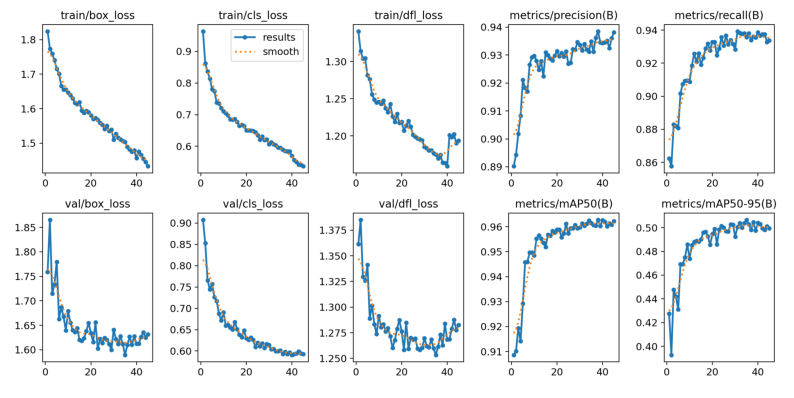
\includegraphics[width=1.0\linewidth]{figures/yolo_scuthead_training_curves.png}
\caption{YOLO training and validation losses and detection metrics (precision, recall, mAP@50, mAP@50--95) across 45 training epochs on the SCUT-Head dataset.}
\label{fig:yolo_training_curves}
\end{figure}

Figure~\ref{fig:yolo_training_curves} shows the training and validation losses together with the main detection metrics across the 45 training epochs. All three training losses decrease consistently throughout the 45-epoch schedule, whereas the corresponding validation losses each reach a minimum earlier in training and subsequently fluctuate within a narrow band without further sustained improvement. This indicates that the model achieves most of its generalisation performance before the end of training, with later training mainly improving the fit to the training data.

\begin{longtable}{p{3.9cm} p{1.4cm} p{1.4cm} p{1.4cm} p{1.4cm} p{1.4cm} p{1.8cm}}
\caption{YOLO training progression on SCUT-Head at key epochs.}
\label{tab:yolo_training_summary} \\

\hline
\centering Epoch &
\centering Train Box &
\centering Val Box &
\centering Precision &
\centering Recall &
\centering mAP@50 &
\centering mAP@50--95 \\
\hline
\endfirsthead

\multicolumn{7}{c}%
{\tablename\ \thetable{} -- continued from previous page} \\
\hline
\centering Epoch &
\centering Train Box &
\centering Val Box &
\centering Precision &
\centering Recall &
\centering mAP@50 &
\centering mAP@50--95 \\
\hline
\endhead

\hline
\multicolumn{7}{r}{Continued on next page} \\
\endfoot

\hline
\endlastfoot

1 (initial)
& 1.8430
& 1.7736
& 0.8840
& 0.8707
& 0.9055
& 0.4227 \\

35 (best mAP@50--95)
& 1.5158
& \textbf{1.5945}
& 0.9290
& 0.9349
& 1.097
& \textbf{0.5057} \\

45 (final)
& \textbf{1.4408}
& 1.6314
& 0.9339
& 0.9335
& 0.9613
& 0.4983 \\

\end{longtable}

As shown in Figure~\ref{fig:yolo_training_curves} and Table~\ref{tab:yolo_training_summary}, the detection metrics reach their best values within a narrow range of epochs, indicating stable convergence. After approximately epoch 35, validation performance shows little further improvement, while training loss continues to decrease. The final epoch remains close to the best performance, suggesting that the additional training was mainly computationally redundant rather than harmful.

\subsubsection{Quantitative Detection-Based Counting Performance}

The fine-tuned YOLO detector shows a substantial improvement in precision, recall, and F1-score on the same 285-image test set, as reported in Table~\ref{tab:yolo_summary}. This improvement results from adapting the model to the head-level annotations, resolving the geometric mismatch identified in Section~\ref{sec:classic_yolo}. The detection metrics remain moderate because head bounding boxes are small, meaning even a small error in box position or size can cause a prediction to fall below the IoU 0.50 threshold. Thus, some remaining errors are related to localisation accuracy rather than complete detection failures.

\begin{longtable}{lc}
\caption{YOLO counting performance on the SCUT-Head test set.}
\label{tab:yolo_summary} \\
\hline
Metric & Value \\
\hline
\endfirsthead

\multicolumn{2}{c}%
{{\tablename\ \thetable{} -- continued from previous page}} \\
\hline
Metric & Value \\
\hline
\endhead

\hline
\multicolumn{2}{r}{{Continued on next page}} \\
\endfoot

\hline
\endlastfoot

Images & 285 \\
Total Ground Truth & 8{,}310 \\
Total Predictions & 7{,}613 \\
True Positives (IoU 0.50) & 3{,}457 \\
False Positives (IoU 0.50) & 4{,}156 \\
False Negatives (IoU 0.50) & 4{,}853 \\
Precision @ IoU 0.50 & 0.4541 \\
Recall @ IoU 0.50 & 0.4160 \\
F1-score @ IoU 0.50 & 0.4342 \\
Mean Ground Truth Count & 29.1579 \\
Mean Predicted Count & 26.7123 \\
Mean Absolute Error (MAE) & 3.3579 \\
Root Mean Squared Error (RMSE) & 4.8778 \\
Mean Absolute Percentage Error (MAPE) & 16.3719\% \\
Pearson Correlation (GT vs.\ Predicted Count) & 0.9725 \\
Coefficient of Determination ($R^2$) & 0.9274 \\

\end{longtable}

The count-level results in Table~\ref{tab:yolo_summary} show that the fine-tuned detector provides more accurate and reliable counting than the pretrained model, with stronger correlation and lower counting errors. The remaining negative counting bias indicates some undercounting, but its reduced magnitude suggests that head-specific training has partially reduced the occlusion-related detection problem. However, performance can still decrease in very dense scenes where heads are heavily occluded.

\begin{figure}[htbp]
\centering
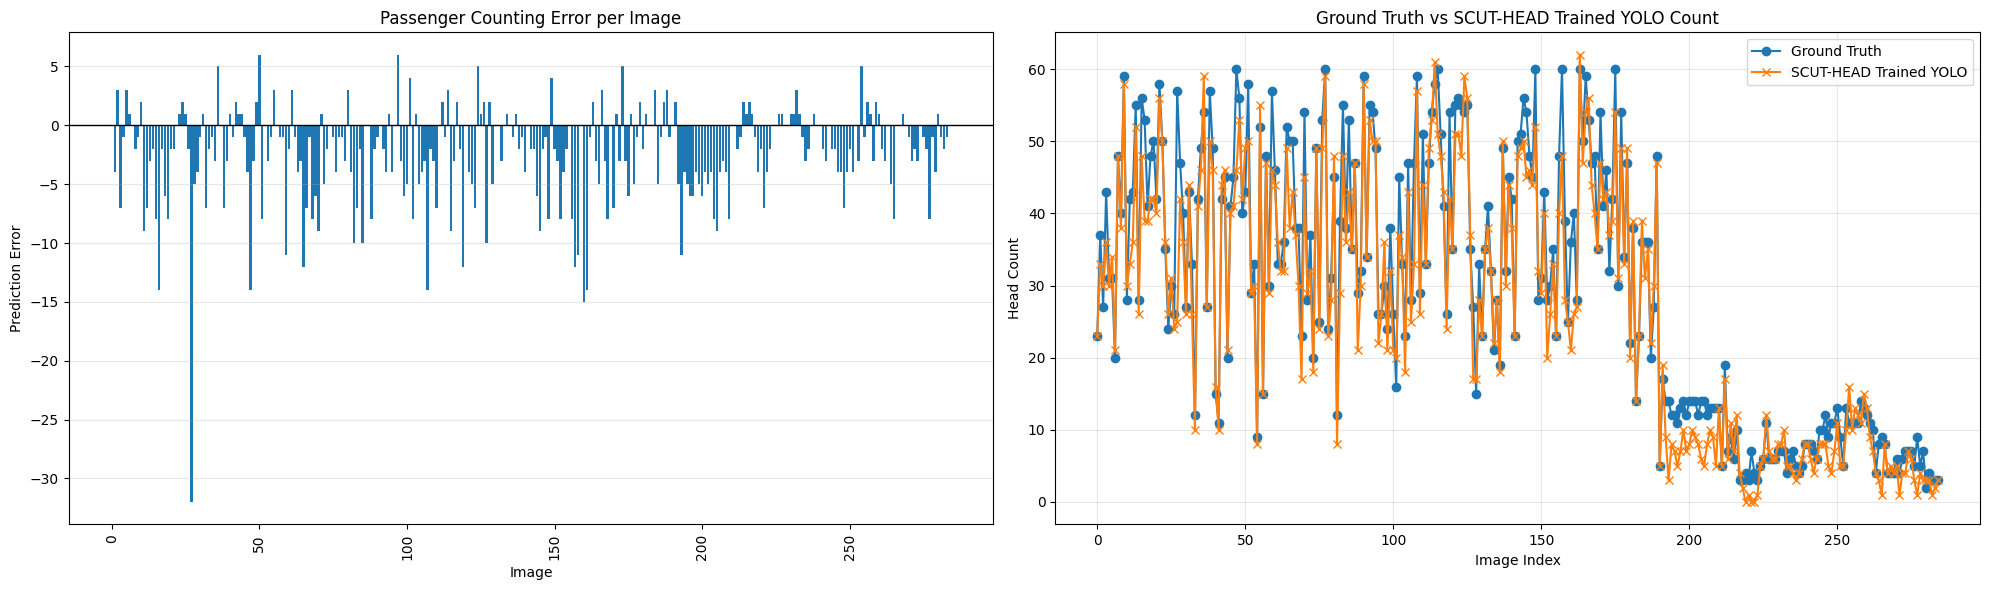
\includegraphics[width=1.0\linewidth]{figures/yolo_scuthead_per_image_error_and_gt_vs_predicted.png}
\caption{Per-image counting error (left) and predicted vs ground-truth counts (right).}
\label{fig:yolo_actual_predicted}
\end{figure}

The largest counting error occurred in a highly crowded image, showing that occlusion remains a limitation even after fine-tuning. The confusion matrix in Figure~\ref{fig:yolo_scuthead_confusion_matrix} further reflects the detector's remaining errors, while the wide variation in per-image F1-scores indicates that detection performance depends strongly on scene density and occlusion conditions.

\begin{figure}[htbp]
\centering
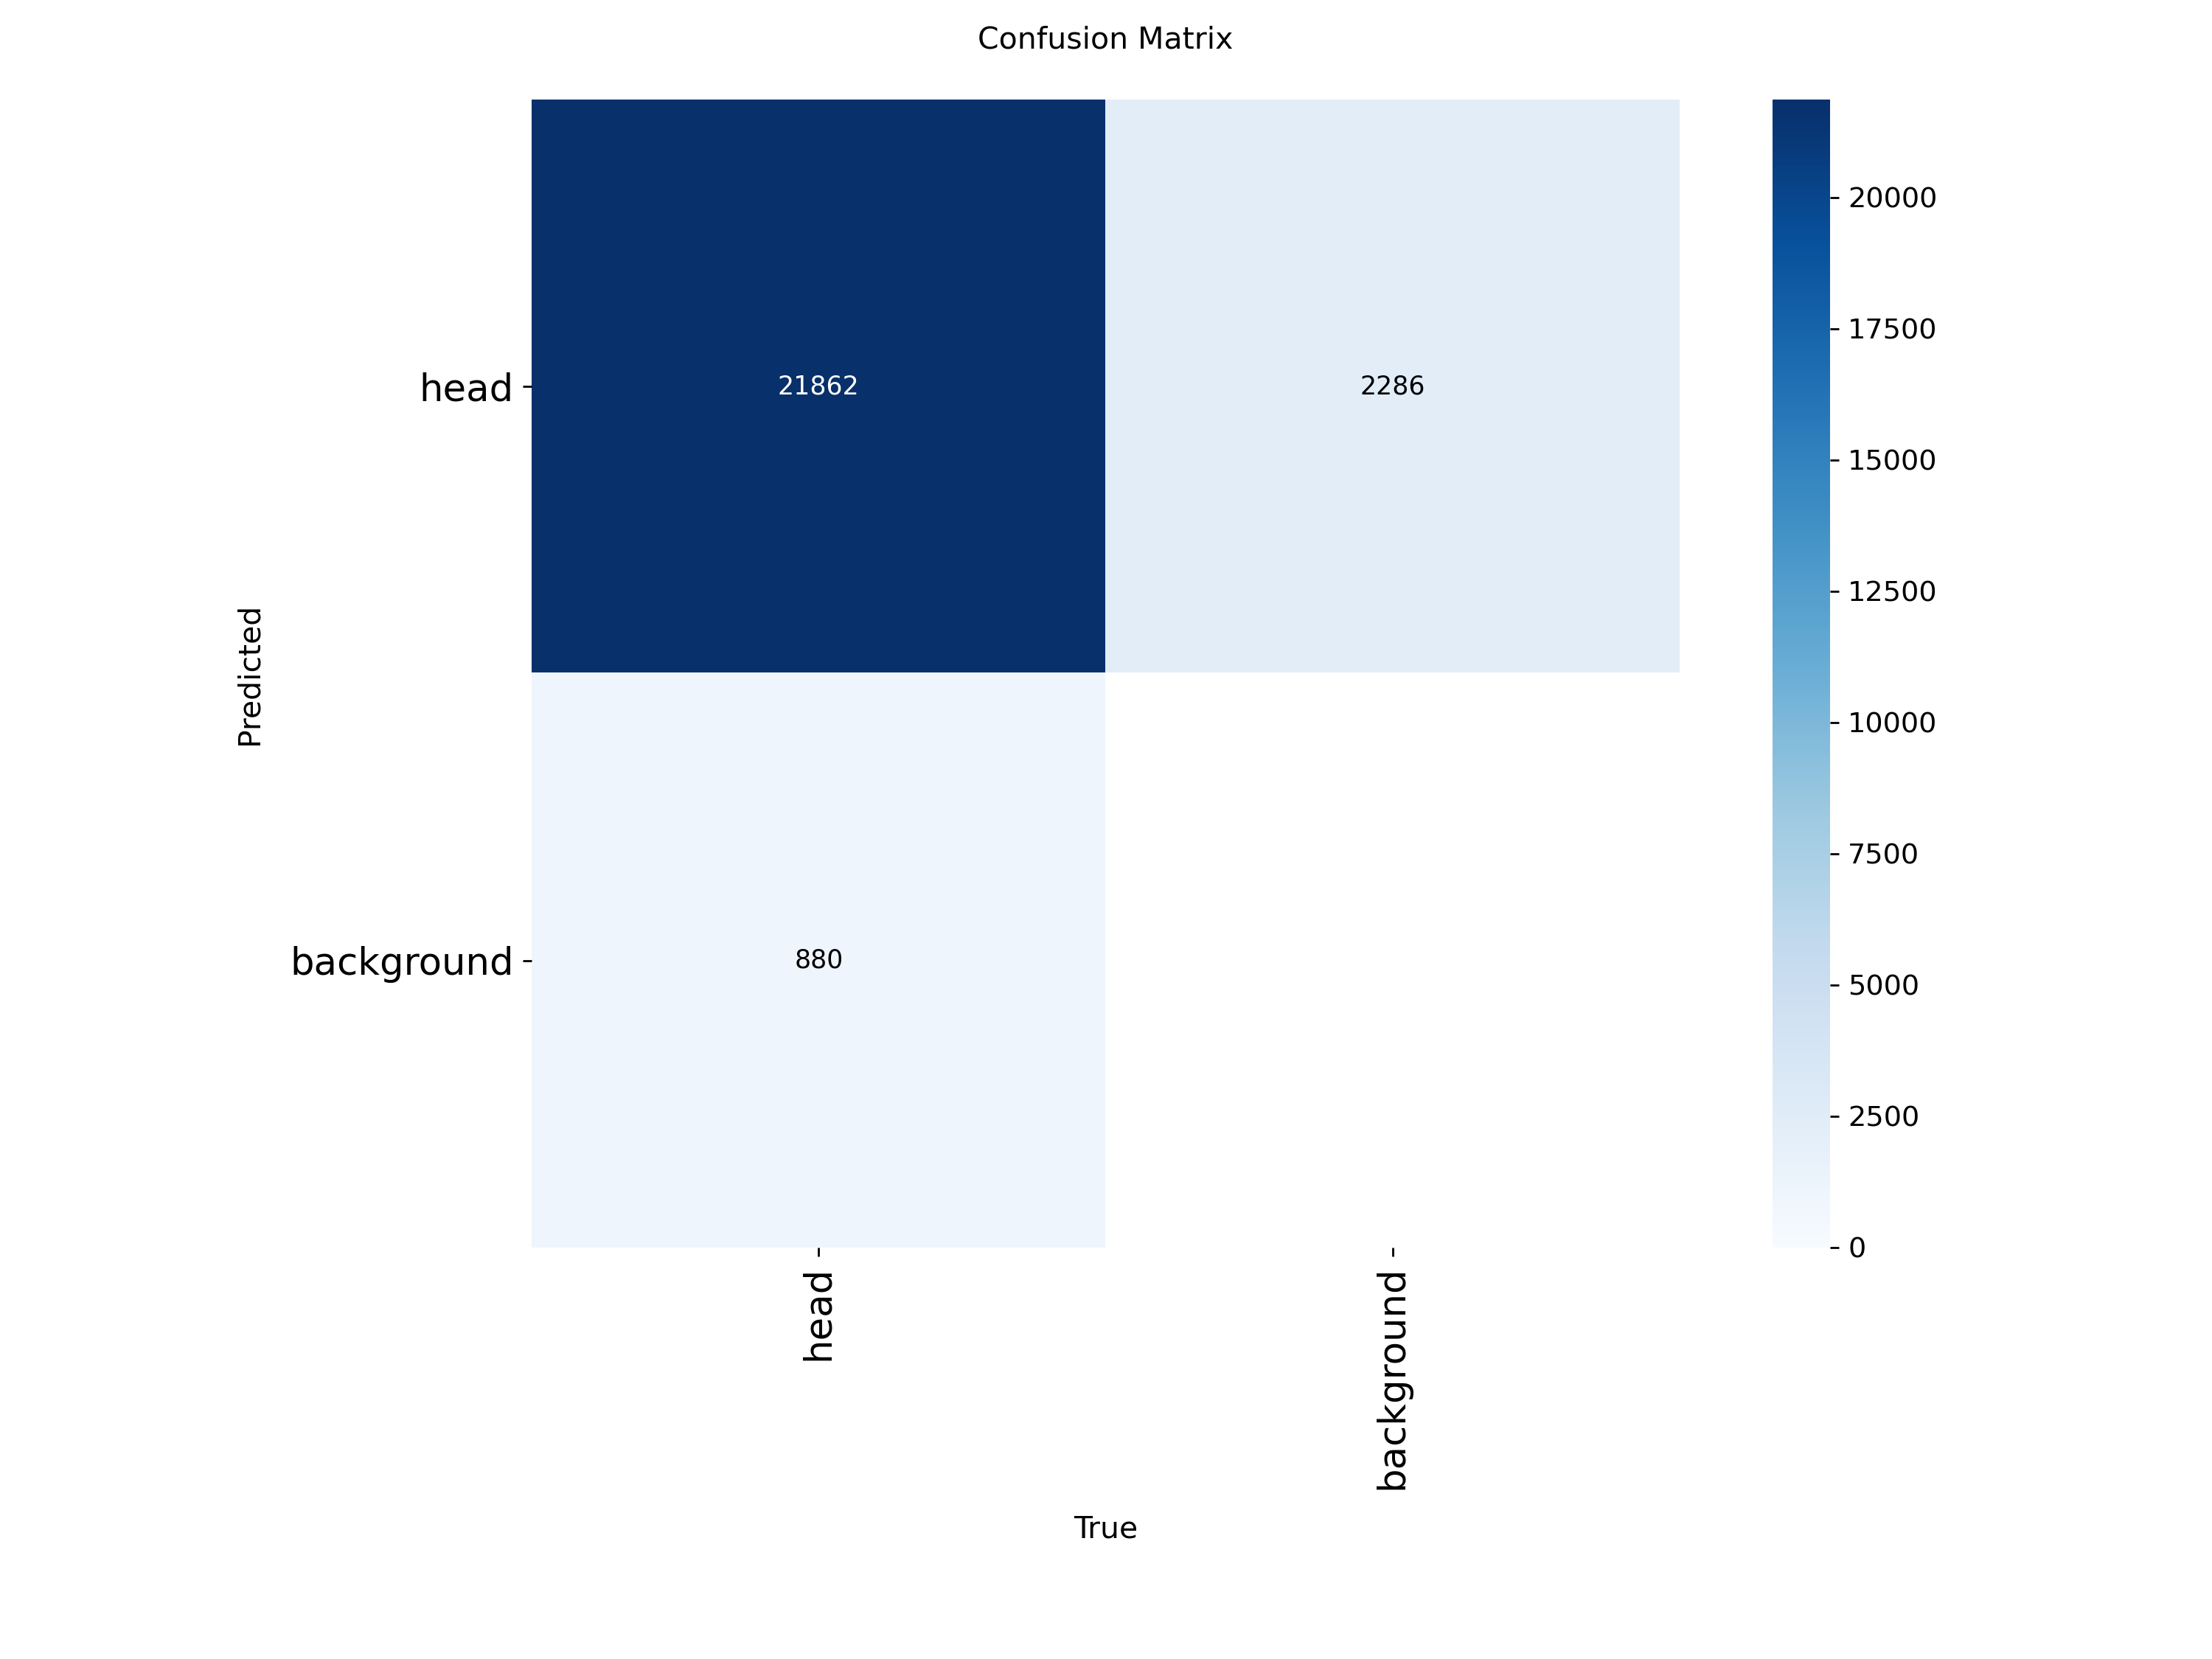
\includegraphics[width=0.7\linewidth]{figures/yolo_scuthead_confusion_matrix.png}
\caption{YOLO head-detector confusion matrix}
\label{fig:yolo_scuthead_confusion_matrix}
\end{figure}

\subsubsection{Detection-Based Counting Performance by Ground-Truth Count Range}

The results in Table~\ref{tab:yolo_range_breakdown} and Figure~\ref{fig:yolo_range_metrics} show that counting performance still depends on crowd density, but is substantially better than the pretrained detector. Absolute error increases as the number of people increases, while relative error and detection quality show clear improvement, especially in low-density scenes. Overall, counting accuracy remains relatively high and stable across moderate- to high-density scenes.

\begin{figure}[htbp]
\centering
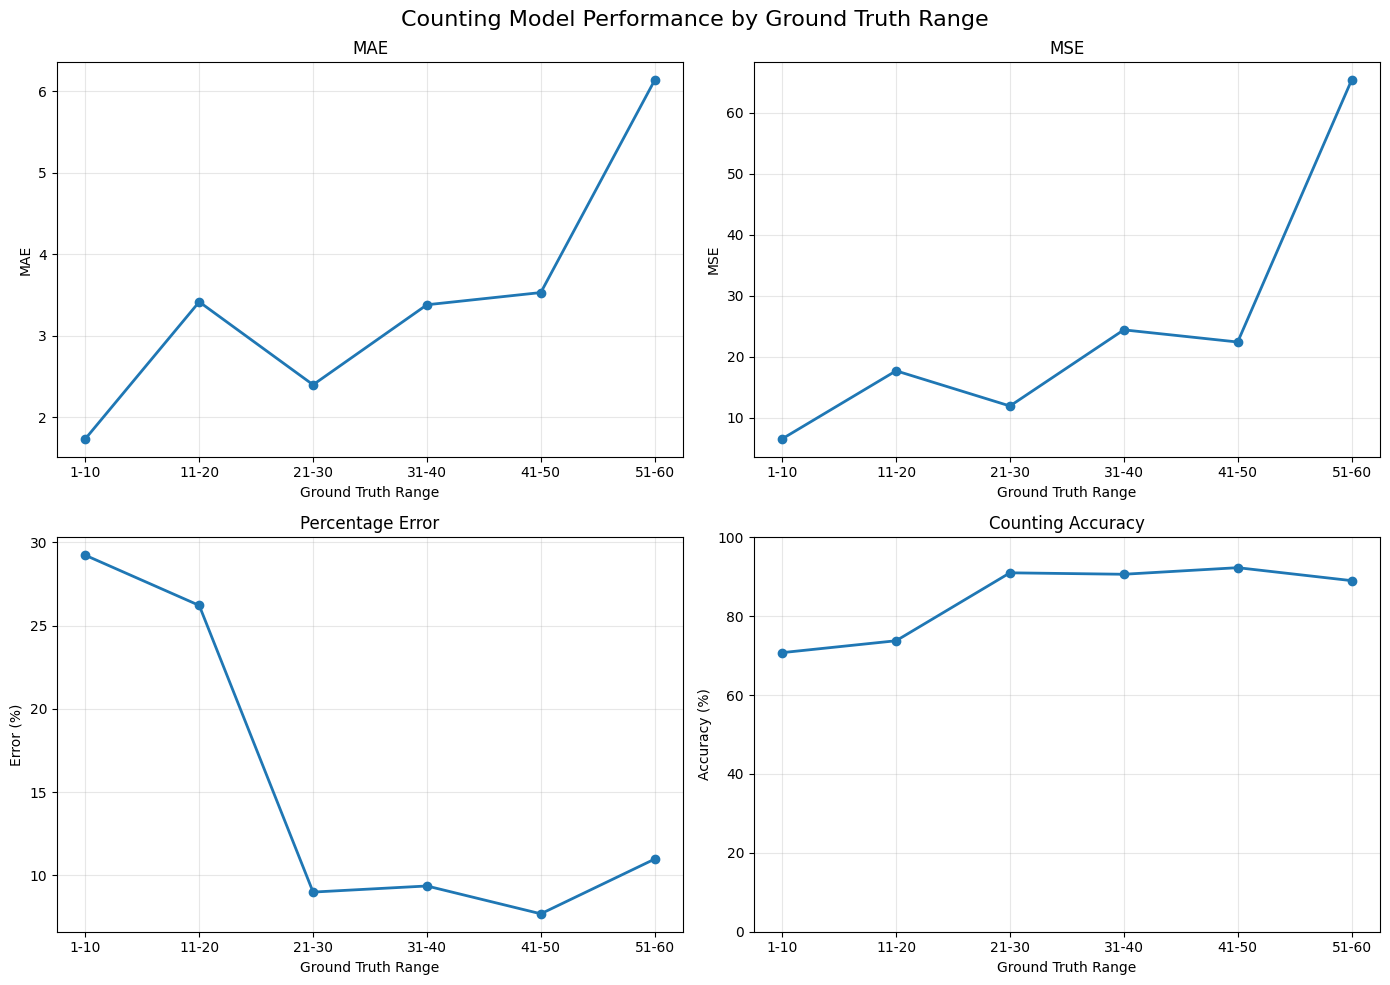
\includegraphics[width=1.0\linewidth]{figures/yolo_scuthead_performance_by_gt_range.png}
\caption{MAE, mean percentage error, mean counting accuracy, and mean detection metrics (precision, recall, F1) of the YOLO detector across ground-truth count ranges.}
\label{fig:yolo_range_metrics}
\end{figure}

The counting bias remains negative across all density ranges and becomes larger as crowd density increases, as shown in Table~\ref{tab:yolo_range_breakdown}. This shows that fine-tuning reduces but does not remove the undercounting caused by occlusion. Figure~\ref{fig:yolo_range_metrics} further illustrates the decline in detection metrics as density increases. When heads are heavily occluded, there is less visible information for the detector to identify them reliably.

\begin{longtable}{lccccccc}
\caption{YOLO head-detector counting performance by ground-truth count range.}
\label{tab:yolo_range_breakdown}\\
\hline
GT Range & $n$ & MAE & RMSE & Mean \% Error & Mean Acc. (\%) & Mean Bias & Mean F1 \\
\hline
\endfirsthead

\multicolumn{8}{c}%
{{\tablename\ \thetable{} -- continued from previous page}} \\
\hline
GT Range & $n$ & MAE & RMSE & Mean \% Error & Mean Acc. (\%) & Mean Bias & Mean F1 \\
\hline
\endhead

\hline
\multicolumn{8}{r}{{Continued on next page}} \\
\endfoot

\hline
\endlastfoot

1--10  & 61 & \textbf{1.7377} & \textbf{2.5543} & 29.2330 & 70.7670 & $-1.2131$ & \textbf{0.5334} \\
11--20 & 48 & 3.4167 & 4.2032 & 26.2192 & 73.7808 & $-2.3750$ & 0.4571 \\
21--30 & 40 & 2.4000 & 3.4496 & \textbf{8.9977} & 91.0023 & $-1.2000$ & 0.4520 \\
31--40 & 42 & 3.3810 & 4.9377 & 9.3644 & 90.6356 & $-2.3810$ & 0.4547 \\
41--50 & 49 & 3.5306 & 4.7316 & 7.6930 & \textbf{92.3070} & $-2.6327$ & 0.4218 \\
51--60 & 45 & 6.1333 & 8.0802 & 10.9798 & 89.0202 & $-5.1556$ & 0.3971 \\

\end{longtable}

These results presented in Table~\ref{tab:yolo_range_breakdown} and Figure~\ref{fig:yolo_range_metrics} show that counting performance depends on crowd density. Counting accuracy is highest in sparse and moderate-density scenes but decreases in high-density scenes, where detection performance also declines. Compared with the pretrained detector, the fine-tuned model has a more predictable failure pattern, but high-density scenes remain challenging. This indicates that detection-based counting has limitations that cannot be fully solved through additional training alone.

\subsection{FourColumn MDNN: Density-Regression Network}
\label{sec:mdnn}

This section reports the experimental results obtained from training and evaluating the proposed MDNN density-estimation model for crowd head counting. The model was trained to learn the relationship between input images and their corresponding density representations, with training and validation performance monitored using loss and mean absolute error (MAE) over 100 epochs. The best-performing checkpoint was selected based on validation performance to provide the most reliable estimate of the model's generalisation capability. The results presented below examine the model's training behaviour, validation performance, and final evaluation results, providing an assessment of its effectiveness for density-based crowd estimation.

\subsubsection{Training Performance and Convergence}

The training history covers 100 epochs and tracks training and validation loss and MAE, along with the best-performing checkpoint. Both training and validation metrics show substantial improvement during training, while training loss and MAE reach their lowest values at the final epoch. In contrast to the detection experiment in Section~\ref{sec:scut_yolo}, the MDNN does not employ a task-specific pretrained backbone, requiring it to learn relevant features directly from the training data. The resulting progression of training and validation performance is presented in Figure~\ref{fig:training_loss}.

\begin{figure}[htbp]
\centering
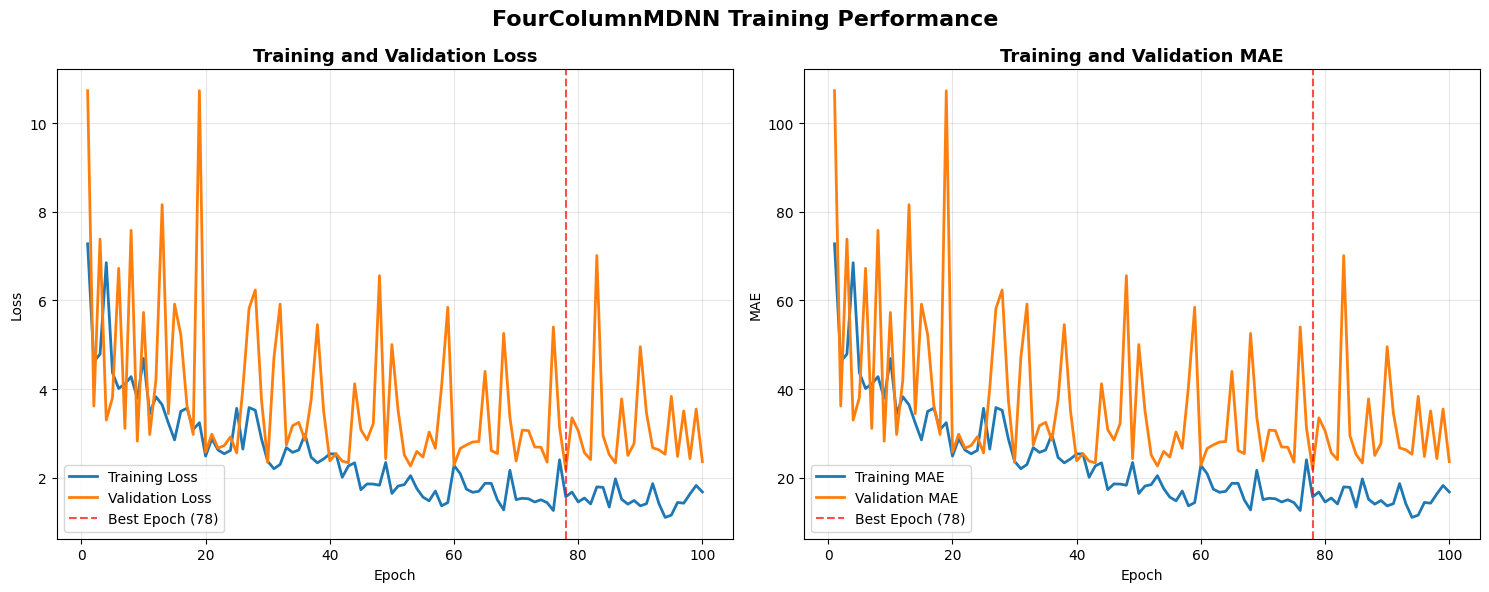
\includegraphics[width=1.0\linewidth]{figures/mdnn_training_validation_loss_mae_curves.png}
\caption{Training and validation loss (left) and MAE (right) across 100 training epochs.}
\label{fig:training_loss}
\end{figure}

The model achieves its best validation performance at epoch 80, with a validation loss of 2.2710 and MAE of 22.6987, as reported in Table~\ref{tab:training_summary}. Although training loss and MAE continue to decrease through epoch 100, the corresponding validation metrics increase to 2.7081 and 27.0703, respectively. This indicates that the model reaches its optimal generalisation performance around epoch 80, after which further training improves the fit to the training data without improving validation performance.

\begin{longtable}{@{\extracolsep{\fill}}lcccc@{}}
\caption{Training progression summary at key epochs.}
\label{tab:training_summary} \\

\hline
\textbf{Epoch} & \textbf{Train Loss} & \textbf{Val Loss} & 
\textbf{Train MAE} & \textbf{Val MAE} \\
\hline
\endfirsthead

\hline
\textbf{Epoch} & \textbf{Train Loss} & \textbf{Val Loss} & 
\textbf{Train MAE} & \textbf{Val MAE} \\
\hline
\endhead

\hline
\multicolumn{5}{r}{\textit{Continued on next page}} \\
\endfoot

\hline
\endlastfoot

1 (initial) 
& 6.6454 
& 9.5432 
& 66.4447 
& 95.4262 \\

80 (best validation) 
& 1.5183 
& \textbf{2.2710} 
& 15.1695 
& \textbf{22.6987} \\

100 (final) 
& \textbf{0.9805} 
& 2.7081 
& \textbf{9.7914} 
& 27.0703 \\

\end{longtable}


Following the best epoch, training loss and training MAE continue to decrease monotonically toward their final values, whereas validation loss and validation MAE fluctuate within a bounded range without falling below their earlier minimum, as evident from Figure~\ref{fig:training_loss} and the key-epoch values reported in Table~\ref{tab:training_summary}. This pattern indicates that the model continues to reduce error on the training set beyond the point of optimal generalisation, without a corresponding improvement on unseen validation data. Consequently, the checkpoint at epoch 80, corresponding to the minimum validation loss and MAE, represents the point of optimal generalisation identified from the recorded training history.


\subsubsection{Quantitative Performance Evaluation}

The aggregate results in Table~\ref{tab:mdnn_summary} are weaker than those of the YOLO-based methods, reflecting the different error characteristics of density-based estimation compared with object detection. The MDNN predicts continuous density maps rather than discrete objects, resulting in only moderate correlation between predicted and ground-truth counts and a negative coefficient of determination. These results suggest limited overall predictive reliability and are examined further through the density-stratified analysis in the following subsection.

\begin{longtable}{@{\extracolsep{\fill}}lc@{}}
\caption{Aggregate MDNN performance on the 285-image test set.}
\label{tab:mdnn_summary} \\

\hline
\textbf{Metric} & \textbf{Value} \\
\hline
\endfirsthead

\hline
\textbf{Metric} & \textbf{Value} \\
\hline
\endhead

\hline
\multicolumn{2}{r}{\textit{Continued on next page}} \\
\endfoot

\hline
\endlastfoot

Images & 285 \\
Total Ground Truth & 8{,}310 \\
Total Predicted & 9{,}659.3860 \\
Mean Ground Truth Count & 29.1579 \\
Mean Predicted Count & 33.8926 \\
Mean Absolute Error (MAE) & 12.9423 \\
Root Mean Squared Error (RMSE) & 18.2807 \\
Mean Absolute Percentage Error (MAPE) & 110.3318\% \\
Pearson Correlation (GT vs.\ Predicted) & 0.5250 \\

\end{longtable}

The MDNN shows a systematic tendency toward overestimation, with the largest percentage errors occurring mainly in images with low ground-truth counts. This pattern is evident in the per-image error distribution shown in Figure~\ref{fig:actual_predicted}, while the aggregate statistics in Table~\ref{tab:mdnn_summary} show a mean predicted count of 33.8926 compared with a mean ground-truth count of 29.1579. This behaviour can be attributed to the model's reliance on local texture and contextual cues rather than explicit object representations, which may cause background patterns or clutter to be interpreted as additional density. Such errors have a greater relative impact in sparse scenes than in densely populated ones, consistent with the largest absolute errors observed in the test set.

\begin{figure}[htbp]
\centering
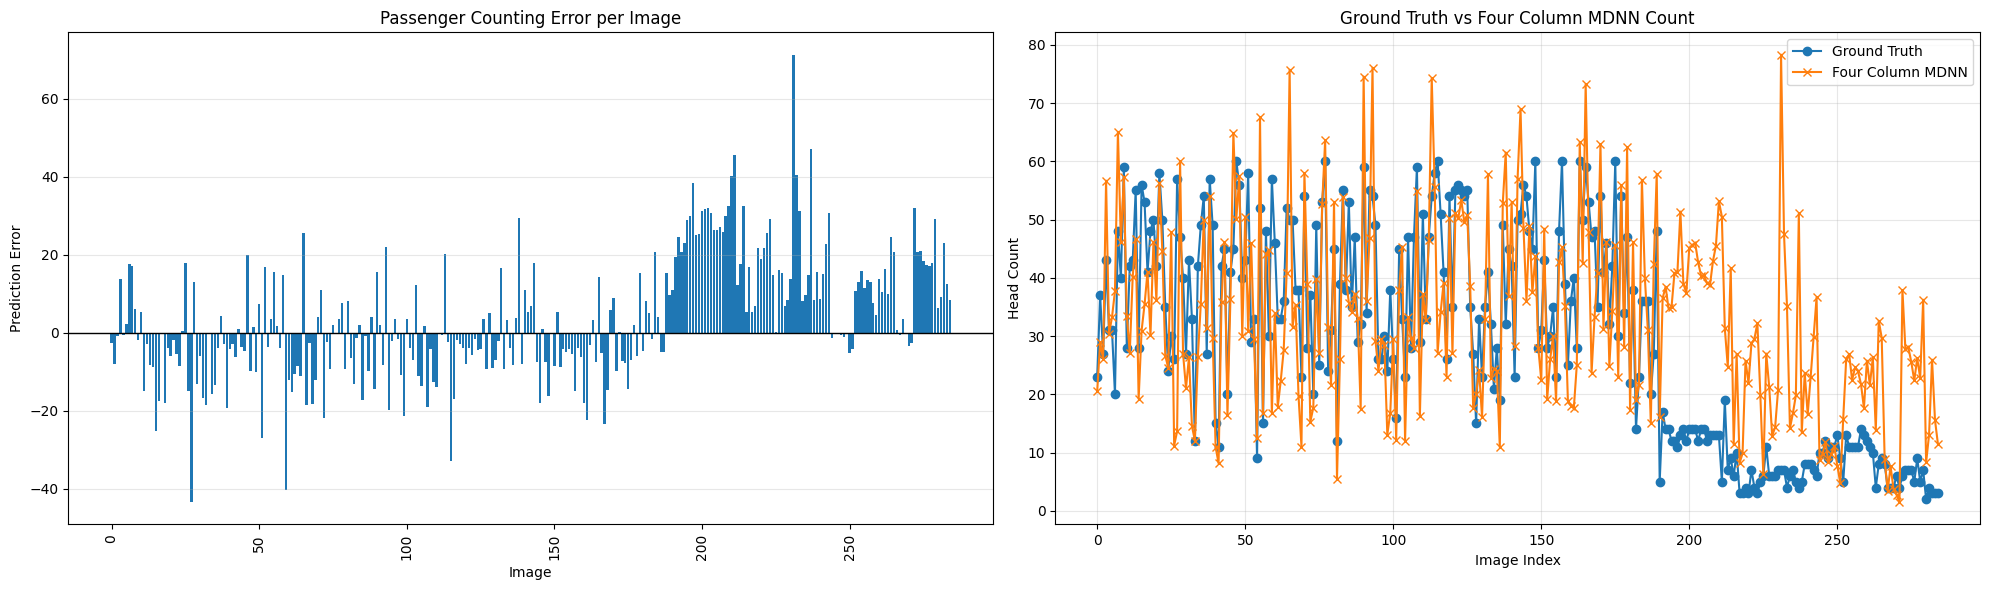
\includegraphics[width=1.0\linewidth]{figures/mdnn_per_image_error_and_gt_vs_predicted.png}
\caption{Per-image counting error (left) and ground-truth versus predicted count (right) across the 285 test images.}
\label{fig:actual_predicted}
\end{figure}

A notable proportion of test images have absolute errors equal to or greater than their ground-truth counts, representing errors comparable to predicting zero. The per-image error plot in Figure~\ref{fig:actual_predicted} illustrates the substantial variation in prediction error across the test set, while the aggregate error statistics in Table~\ref{tab:mdnn_summary} further quantify this variability. This finding supports the identified limitation in sparse scenes, where relatively small amounts of incorrectly attributed background density can produce errors exceeding the actual number of individuals.

\subsubsection{MDNN Performance by Ground-Truth Count Range}

The density-range results in Table~\ref{tab:range_breakdown} and Figure~\ref{fig:range_metrics} clarify the aggregate findings and reveal a pattern opposite to that of the detection-based methods. While detection performance is strongest in sparse scenes and declines with increasing density, MDNN performs poorly at very low counts but improves substantially at moderate densities and remains relatively stable thereafter. This behaviour is consistent with density regression, as stronger crowd-density signals provide more reliable texture and contextual cues, whereas sparse scenes make background-related noise more significant relative to the true count.

\begin{figure}[htbp]
\centering
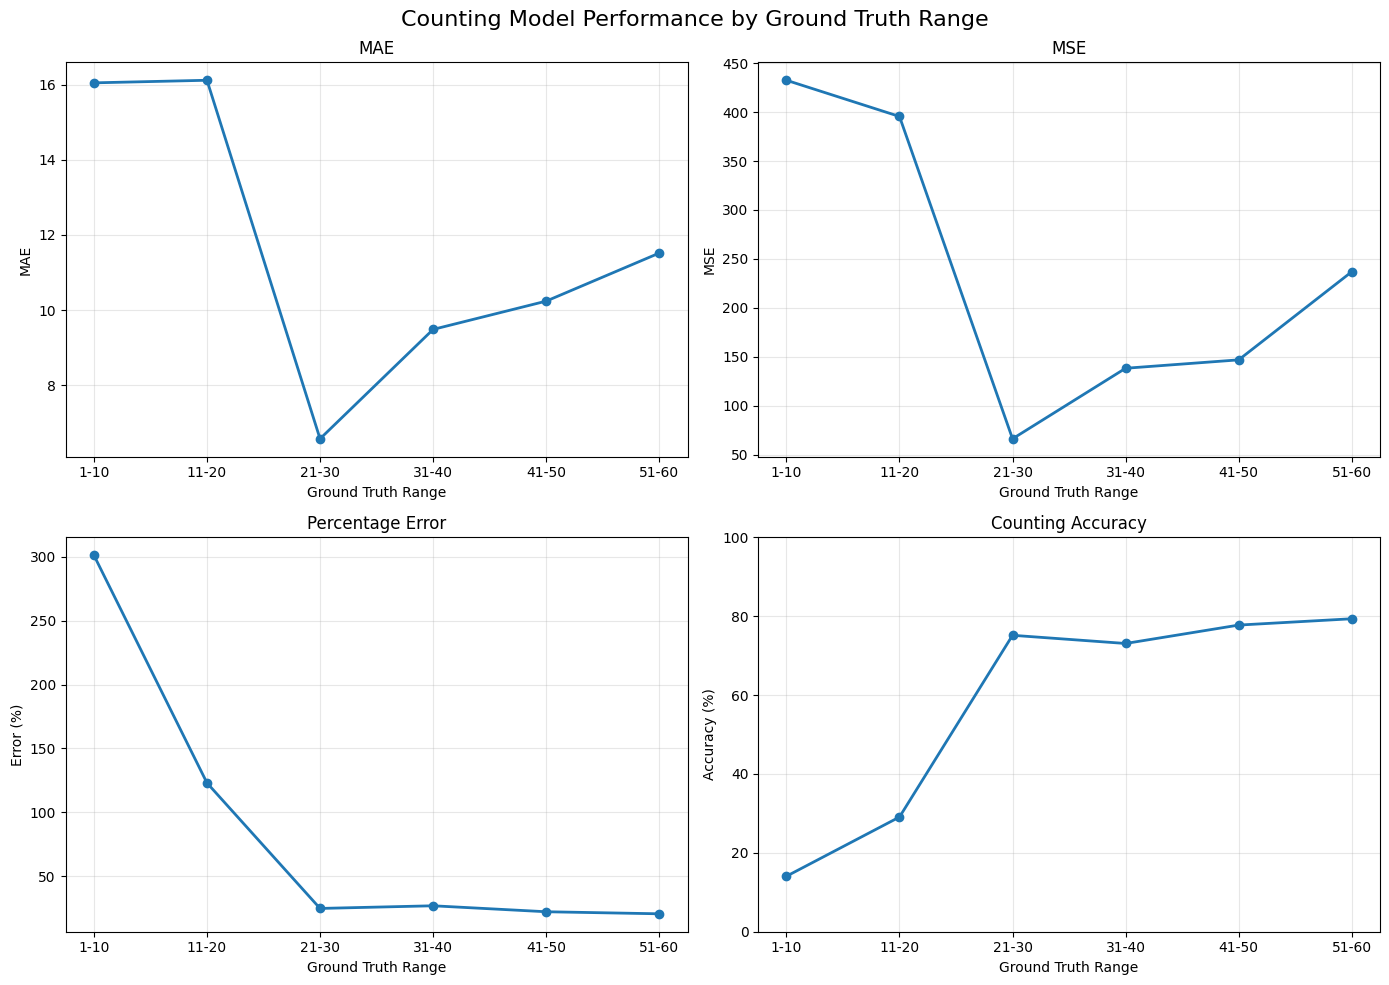
\includegraphics[width=1.0\linewidth]{figures/mdnn_performance_by_gt_range.png}
\caption{MAE, MSE, mean percentage error, and mean counting accuracy of the MDNN across ground-truth count ranges.}
\label{fig:range_metrics}
\end{figure}

The bias also varies with crowd density, supporting the above interpretation. It is strongly positive in the sparsest scenes, indicating overestimation likely caused by background and textural noise, but becomes mildly negative for counts above approximately 20, suggesting moderate underestimation as crowd density increases. This may result from overlapping and closely spaced individuals producing compressed density representations that are more difficult for the network to distinguish accurately.

\begin{longtable}{@{\extracolsep{\fill}}lccccc c@{}}
\caption{MDNN prediction performance by ground-truth count range (bin width = 10).}
\label{tab:range_breakdown} \\
\hline
GT Range & $n$ & MAE & RMSE & Mean \% Error & Mean Accuracy (\%) & Mean Bias \\
\hline
\endfirsthead

\hline
GT Range & $n$ & MAE & RMSE & Mean \% Error & Mean Accuracy (\%) & Mean Bias \\
\hline
\endhead

\hline
\endfoot

\hline
\endlastfoot

1--10  & 61 & 18.4675 & 26.8621 & 345.3091 & 15.4442 & 17.9646 \\
11--20 & 48 & 16.2676 & 21.2526 & 123.7618 & 36.2343 & 14.7079 \\
21--30 & 40 & \textbf{7.0901} & \textbf{8.7197} & \textbf{26.9140} & 73.0860 & \textbf{$-0.8633$} \\
31--40 & 42 & 10.7568 & 13.0606 & 30.3733 & 69.6267 & $-3.5655$ \\
41--50 & 49 & 11.5492 & 14.1557 & 25.1219 & 74.8893 & $-2.0146$ \\
51--60 & 45 & 10.6642 & 14.5467 & 19.0432 & \textbf{81.068} & $-3.7653$ \\

\end{longtable}

Taken together with the range-based results of the two detection-based methods, these findings provide strong empirical support for combining detection- and density-based counting in a single adaptive framework. MDNN performs least reliably in sparse scenes, where detection-based methods are strongest, while its performance becomes more stable at higher densities, where detection methods are increasingly affected by occlusion. Thus, the two approaches exhibit complementary strengths across different crowd-density conditions rather than differing solely in overall accuracy.

\subsection{CSRNet: VGG-16-Based Density-Regression Network}
\label{sec:csrnet}

This section reports the experimental results obtained from training and evaluating CSRNet for crowd head counting on the same 285-image test set used throughout this chapter. Similar to the proposed MDNN described in Section~\ref{sec:mdnn}, CSRNet estimates a continuous density map and derives the final crowd count by integrating the predicted density rather than explicitly localising individual heads. The two networks therefore represent alternative implementations of the density-based counting paradigm and can be compared directly in terms of their training behaviour, aggregate counting accuracy, and performance across different crowd-density ranges.

\subsubsection{Training Performance and Convergence}

The CSRNet training history covers 100 epochs and records training and validation loss and MAE under a step-decayed learning-rate schedule. The learning rate is initially set to $1\times10^{-4}$ and is reduced by an order of magnitude at epochs 87, 92, and 97, reaching a final value of $1\times10^{-7}$. As illustrated in Figure~\ref{fig:csrnet_training_curves}, both training and validation loss decrease rapidly during the early stages of training and then converge gradually as training progresses. The learning-rate reductions near the end of the schedule produce only small additional changes in the validation metrics, indicating that the model has largely stabilised before the final epoch.

\begin{figure}[htbp]
\centering

\includegraphics[width=1.0\linewidth]{figures/csrnet_training_validation_loss_mae_curves.png}
\caption{CSRNet training and validation loss (left) and MAE (right) across 100 training epochs.}
\label{fig:csrnet_training_curves}
\end{figure}

Figure~\ref{fig:csrnet_training_curves} shows that CSRNet converges substantially during the early epochs, followed by a gradual reduction in both training and validation error. Unlike the MDNN, for which the validation performance reaches its best point at epoch 80 and subsequently deteriorates despite continued improvement in the training metrics, CSRNet maintains a close correspondence between its training and validation curves during the later stages of training. The key training values are summarised in Table~\ref{tab:csrnet_training_summary}.

\begin{longtable}{@{\extracolsep{\fill}}lcccc@{}}
\caption{CSRNet training progression at key epochs.}
\label{tab:csrnet_training_summary} \

\hline
\textbf{Epoch} & \textbf{Train Loss} & \textbf{Val Loss} &
\textbf{Train MAE} & \textbf{Val MAE} \
\hline
\endfirsthead

\hline
\textbf{Epoch} & \textbf{Train Loss} & \textbf{Val Loss} &
\textbf{Train MAE} & \textbf{Val MAE} \
\hline
\endhead

\hline
\multicolumn{5}{r}{\textit{Continued on next page}} \
\endfoot

\hline
\endlastfoot

1 (initial)
& 576.6667
& 19.6584
& 8.9699
& 3.3617 \

99 (best validation)
& 0.0015
& \textbf{0.0035}
& 0.0139
& \textbf{0.0173} \

100 (final)
& \textbf{0.0014}
& 0.0035
& \textbf{0.0140}
& 0.0172 \

\end{longtable}

The final training and validation metrics remain closely aligned, with the train--validation MAE difference remaining below approximately 0.003 during the last 20 epochs, as indicated by Figure~\ref{fig:csrnet_training_curves}. This behaviour suggests that CSRNet does not exhibit the same degree of post-optimal training divergence observed for MDNN. Instead, the model reaches a stable solution in which further reductions in training error produce little change in validation performance. The substantially smaller loss and MAE values compared with the count-level errors reported in Table~\ref{csrnet_training_summary} also indicate that the training metrics are associated with normalised or rescaled density targets and should therefore be interpreted primarily as indicators of optimisation behaviour rather than as direct measures of image-level counting error.

Compared with MDNN, CSRNet therefore demonstrates a more stable training trajectory. MDNN continues to reduce its training error after its best validation checkpoint at epoch 80, whereas CSRNet's training and validation metrics remain closely coupled toward the end of training. This indicates that CSRNet achieves a comparatively stable convergence pattern, although the stability of the training process does not by itself imply high counting accuracy on unseen test images.

\subsubsection{Quantitative Performance Evaluation}

The aggregate CSRNet results are presented in Table~\ref{csrnet_training_summary}. Compared with the MDNN results in Table~\ref{tab:mdnn_summary}, CSRNet achieves lower MAE, RMSE, and MAPE, together with a slightly higher Pearson correlation and a positive coefficient of determination. These results indicate that CSRNet provides a modest overall improvement in count prediction relative to MDNN. However, the correlation remains weak and the overall errors remain substantial, showing that the improvement does not translate into consistently accurate predictions across the complete test set.

\begin{longtable}{@{\extracolsep{\fill}}lc@{}}
\caption{Aggregate CSRNet performance on the 285-image test set.}
\label{csrnet_training_summary} \\

\hline
\textbf{Metric} & \textbf{Value} \\
\hline
\endfirsthead

\hline
\textbf{Metric} & \textbf{Value} \\
\hline
\endhead

\hline
\multicolumn{2}{r}{\textit{Continued on next page}} \\
\endfoot

\hline
\endlastfoot

Images & 285 \\
Total Ground Truth & 8{,}310 \\
Total Predicted & 9{,}216.0216 \\
Mean Ground Truth Count & 29.1579 \\
Mean Predicted Count & 32.3369 \\
Mean Absolute Error (MAE) & 10.6559 \\
Root Mean Squared Error (RMSE) & 17.7773 \\
Mean Absolute Percentage Error (MAPE) & 93.6675\% \\
Pearson Correlation (GT vs.\ Predicted) & 0.5539 \\
Coefficient of Determination ($R^2$) & 0.0354 \\

\end{longtable}

The per-image prediction behaviour is illustrated in Figure~\ref{fig:csrnet_actual_predicted}, which shows the counting error for individual test images together with the relationship between ground-truth and predicted counts. The figure demonstrates that, despite the improvement in aggregate metrics, substantial variation remains between individual predictions.

\begin{figure}[htbp]
\centering
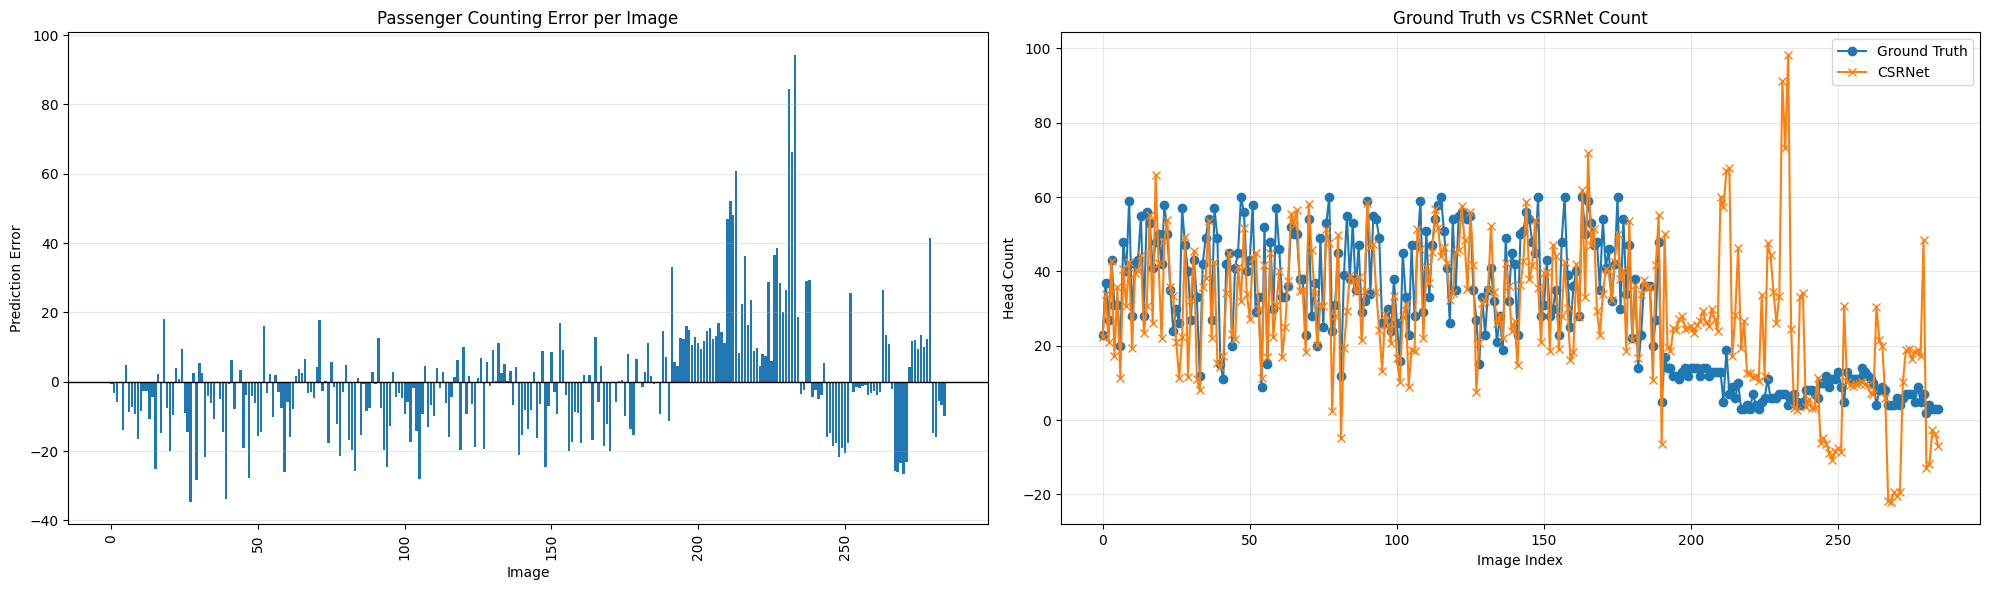
\includegraphics[width=1.0\linewidth]{figures/csrnet_per_image_error_and_gt_vs_predicted.png}
\caption{Per-image counting error (left) and ground-truth versus predicted count (right) across the 285 CSRNet test images.}
\label{fig:csrnet_actual_predicted}
\end{figure}

As shown in Figure~\ref{fig:csrnet_actual_predicted}, CSRNet exhibits a systematic tendency toward overestimation, with the mean predicted count of 32.3369 exceeding the mean ground-truth count of 29.1579 by approximately 3.18 individuals, as reported in Table~\ref{csrnet_training_summary}. The most extreme error is also associated with a sparse scene: the model overestimates a ground-truth count of 4 by 127.18 individuals. Furthermore, 62 of the 285 test images (21.8\%) have an absolute error at least as large as the corresponding ground-truth count. This indicates that, despite its improved aggregate performance over MDNN, CSRNet retains a substantial vulnerability to large counting errors in sparse scenes.

The comparison with MDNN is therefore mixed. CSRNet improves the aggregate MAE from 12.9423 to 10.6559 and the Pearson correlation from 0.5250 to 0.5539, while also changing the coefficient of determination from the negative value obtained by MDNN to a slightly positive $R^2$ of 0.0354. However, both networks exhibit the same general tendency toward overestimation in sparse scenes. The results therefore suggest that CSRNet improves the overall density estimation process without eliminating the principal failure mode identified for MDNN.

\subsubsection{CSRNet Performance by Ground-Truth Count Range}

To examine whether the aggregate improvement of CSRNet is consistent across different crowd densities, its performance is evaluated using the same ground-truth count ranges applied to MDNN and the two YOLO-based methods. Table~\ref{tab:csrnet_range_breakdown} and Figure~\ref{fig:csrnet_range_metrics} show the resulting density-stratified performance.

\begin{figure}[htbp]
\centering

\includegraphics[width=1.0\linewidth]{figures/csrnet_range_metrics.png}
\caption{CSRNet performance across ground-truth count ranges, showing MAE, RMSE, mean percentage error, mean accuracy, and mean bias.}
\label{fig:csrnet_range_metrics}
\end{figure}

Figure~\ref{fig:csrnet_range_metrics} shows a clear dependence of CSRNet performance on ground-truth crowd density. The largest errors occur in the sparsest range of 1--10 individuals, while the error decreases substantially in the moderate-density ranges. Performance then remains comparatively stable at higher counts. This pattern is broadly consistent with the behaviour observed for MDNN in Figure~\ref{fig:range_metrics}, although CSRNet generally achieves lower errors in the moderate-density regime.

\begin{longtable}{@{\extracolsep{\fill}}lcccccc@{}}
\caption{CSRNet prediction performance by ground-truth count range (bin width = 10).}
\label{tab:csrnet_range_breakdown} \\

\hline
\textbf{GT Range} & \textbf{$n$} & \textbf{MAE} & \textbf{RMSE} &
\textbf{Mean \% Error} & \textbf{Mean Accuracy (\%)} & \textbf{Mean Bias} \\
\hline
\endfirsthead

\hline
\textbf{GT Range} & \textbf{$n$} & \textbf{MAE} & \textbf{RMSE} &
\textbf{Mean \% Error} & \textbf{Mean Accuracy (\%)} & \textbf{Mean Bias} \\
\hline
\endhead

\hline
\multicolumn{7}{r}{\textit{Continued on next page}} \\
\endfoot

\hline
\endlastfoot

1--10
& 61
& 15.1607
& 29.7167
& 302.3687
& 20.1351
& 14.9335 \\

11--20
& 48
& \textbf{11.7854}
& \textbf{16.0560}
& \textbf{90.5073}
& 32.2793
& 10.5074 \\

21--30
& 40
& 7.5173
& 9.6618
& 29.0258
& 71.0124
& $-0.6292$ \\

31--40
& 42
& 7.4371
& 10.7183
& 21.0074
& 79.0589
& $-3.1704$ \\

41--50
& 49
& 9.8036
& 13.3726
& 21.3963
& 78.9686
& $-1.0126$ \\

51--60
& 45
& 10.0668
& 12.0234
& 18.1028
& \textbf{81.8972}
& $-6.6964$ \\

\end{longtable}

The comparison with MDNN in Table~\ref{tab:range_breakdown} shows that CSRNet's overall advantage is concentrated mainly in the moderate-density ranges. In the 11--20 range, CSRNet reduces MAE from 16.2676 to 11.7854 and RMSE from 21.2526 to 16.0560. Similar improvements are observed in the 31--40 and 41--50 ranges. In the 21--30 range, the two networks perform comparatively similarly, with MDNN achieving a slightly lower MAE of 7.0901 compared with CSRNet's 7.5173.

The density-stratified results therefore show that CSRNet improves upon MDNN primarily when a moderate density signal is present. At low counts, neither density-regression architecture provides the reliability achieved by the detection-based methods. This supports the density-adaptive interpretation developed in Section~\ref{sec:mdnn}: detection-based counting is better suited to sparse scenes, while density-based methods become more competitive as crowd density increases and individual localisation becomes more difficult.